\documentclass{beamer}
% Try the class options [notes], [notes=only], [trans], [handout],
% [red], [compress], [draft] and see what happens!

% \usepackage{definitions}
\usepackage[british]{babel}
\usepackage{color, soul}
\usepackage{tikz}

%% tikz tricks
% \tikzset{onslide/.code args={<#1>#2}{%
%   \only<#1>{\pgfkeysalso{#2}} 
% }}

\pdfinfo{
        /Title (cim)
        /Creator (LaTeX)
        /Producer (pdflatex)
        /Author (szerzo)
        /CreationDate (datum)
	/Subject (tema)
}


\mode<article> % only for the article version
{
  \usepackage{fullpage}
  \usepackage{hyperref}
}
\mode<presentation>
{
  \usetheme[left,width=0.65in,height=0.55in]{Kolozsvar}
  \setbeamercovered{transparent}
  \setbeamertemplate{navigation symbols}{}
  \setbeamertemplate{footline}%
     {\vspace*{-1.4em}\hspace*{0.66in}\textbf{\insertframenumber/\inserttotalframenumber}\newline\vspace*{0.4em}}
		\setbeamerfont{block title}{size=\larger} % RELSIZE -- html-sizes 
		\usefonttheme{professionalfonts}
		\setbeamercolor{math text}{fg=green!30!red!30!brown}
		\setbeamercolor{normal text in math text}{parent=math text}
}

\setbeamercovered{dynamic}

% The following info should normally be given in you main file:
\title[Apache Kafka]{Apache Kafka}
%
\author{ Hunor Ördög, Norbert-Raymond Pap}
%
\institute[UBB Cluj-Napoca]{
  Department of Mathematics and Informatics\\
  Babe{\c{s}}--Bolyai University, Cluj-Napoca}
%
\date{2024 May}


\begin{document}

\frame{\maketitle}

\mode<presentation>
{
  % \begin{frame}
  %   \frametitle{Talk structure}
  % \tableofcontents
  % \end{frame} 

  % \AtBeginSection[]
  {
      \begin{frame}<beamer>{Contents}
        % \tableofcontents[currentsection,currentsubsection,hideothersubsections]
        \tableofcontents
      \end{frame}
    }
}

%%%%%%%%%%%%%%%%%%%%%%%%%%%%%%%%%%%%%%%%%%%%%%%%%%%%%%%%%%%%%%%%%%%%%%
\section[What is Kafka?]{What is Kafka?}

\begin{frame}{What is Kafka?}
  
\includegraphics[scale=0.25]{fig/kafka_logo.png}
  \vspace*{2em}
  \begin{itemize}
    \item Open-source \underline{distributed event streaming platform}.
  \end{itemize}
\end{frame}

\begin{frame}{What is a “distributed streaming platform”?}
  \begin{itemize}
    \item Streams are just infinite data, data that never ends.
    \item Distributed means Kafka works in a cluster, each node in the cluster is called a \textbf{Broker}.
          % Brokers are just servers executing a copy of apache kafka.
          \vspace*{1em}
    \item Kafka is a set of machines working together to be able to handle and process real-time infinite data.
  \end{itemize}
\end{frame}


\begin{frame}{Where does Kafka come from?}
  \begin{itemize}
    \item Kafka was originally developed at LinkedIn 
\includegraphics[scale=0.006]{fig/linkedin_logo.png} in 2010
    \item Open sourced in early 2011
  \end{itemize}
  \vspace*{1em}
  \hspace*{3.1em}
  
\includegraphics[scale=0.17]{fig/apache_software.png}
\end{frame}
% 2012 ota Apache Kafka neven ismert es azota ok tartsak karban

\section[Kafka components \& Internal Architecture]{Kafka components \& Internal Architecture}

\begin{frame}{Kafka Components}
  \begin{itemize}
    \item Producer
    \item Consumer
    \item Broker
    \item Cluster
    \item Topic
    \item Partitions
    \item Offset
    \item Consumer Groups
    \item Zookeeper
  \end{itemize}
  \begin{tikzpicture}[remember picture, overlay]
    \node[left=3em] at (current page.east)
    {
      
\includegraphics[width=0.35\textwidth]{fig/kafka_logo.png}
    };
  \end{tikzpicture}
\end{frame}

\begin{frame}{Kafka Components}
  \begin{itemize}
    \item \hl{Producer}
    \item Consumer
    \item Broker
    \item Cluster
    \item Topic
    \item Partitions
    \item Offset
    \item Consumer Groups
    \item Zookeeper
  \end{itemize}
  \begin{tikzpicture}[remember picture, overlay]
    \node[left=3em] at (current page.east)
    {
      
\includegraphics[width=0.35\textwidth]{fig/kafka_logo.png}
    };
  \end{tikzpicture}
\end{frame}

\begin{frame}{Kafka Components}{Producer}
  \begin{itemize}
    \item A producer is the source of data who will publish events.
  \end{itemize}
  \vspace*{1.5em}
  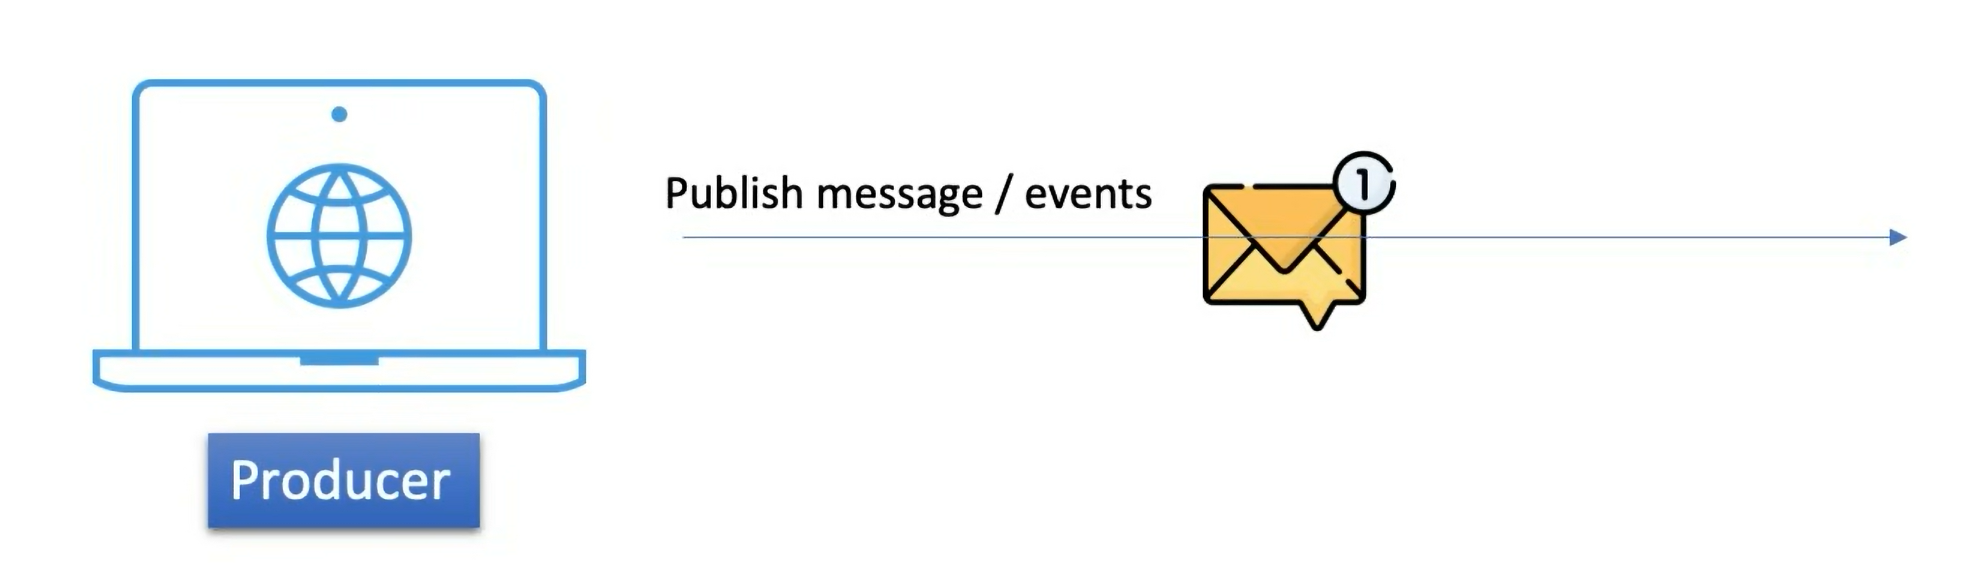
\includegraphics[scale=0.192]{fig/producer.png}
\end{frame}

\begin{frame}{Kafka Components}
  \begin{itemize}
    \item Producer
    \item \hl{Consumer}
    \item Broker
    \item Cluster
    \item Topic
    \item Partitions
    \item Offset
    \item Consumer Groups
    \item Zookeeper
  \end{itemize}
  \begin{tikzpicture}[remember picture, overlay]
    \node[left=3em] at (current page.east)
    {
      
\includegraphics[width=0.35\textwidth]{fig/kafka_logo.png}
    };
  \end{tikzpicture}
\end{frame}

\begin{frame}{Kafka Components}{Consumer}
  \begin{itemize}
    \item A consumer acts as a receiver, consumes events.
  \end{itemize}
  \vspace*{1.5em}
  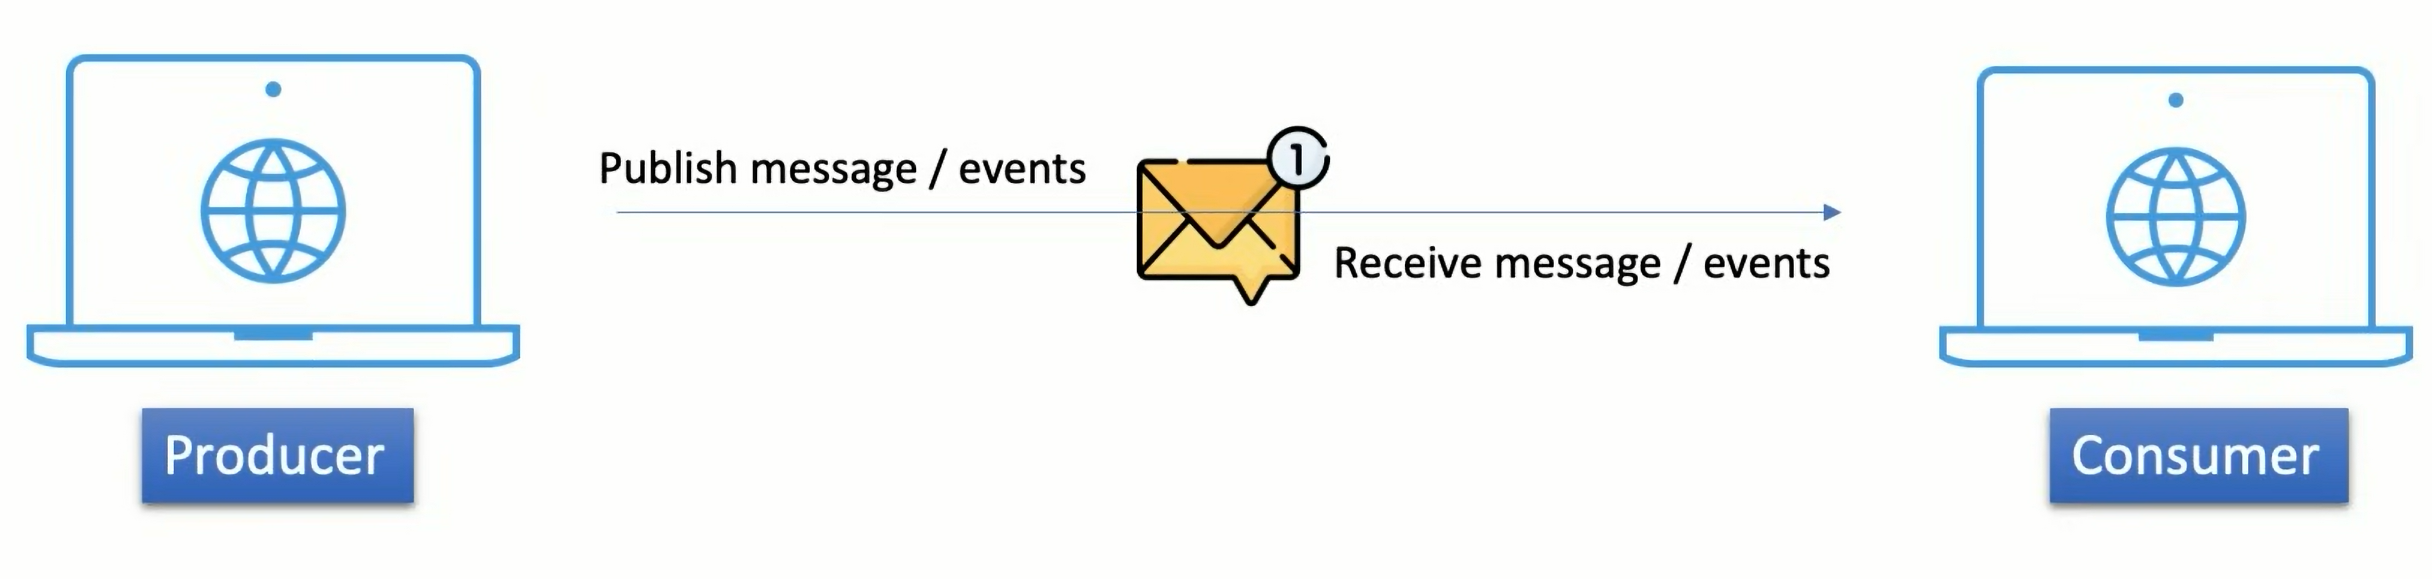
\includegraphics[scale=0.16]{fig/consumer.png}
\end{frame}

\begin{frame}{Kafka Components}
  \begin{itemize}
    \item Producer
    \item Consumer
    \item \hl{Broker}
    \item Cluster
    \item Topic
    \item Partitions
    \item Offset
    \item Consumer Groups
    \item Zookeeper
  \end{itemize}
  \begin{tikzpicture}[remember picture, overlay]
    \node[left=3em] at (current page.east)
    {
      
\includegraphics[width=0.35\textwidth]{fig/kafka_logo.png}
    };
  \end{tikzpicture}
\end{frame}

\begin{frame}{Kafka Components}{Broker}
  \begin{itemize}
    \item The Kafka Broker is the Kafka server.
    \item A broker is an intermediate entity that helps in message exchanges between producers and consumers.
  \end{itemize}
  \vspace*{1.5em}
  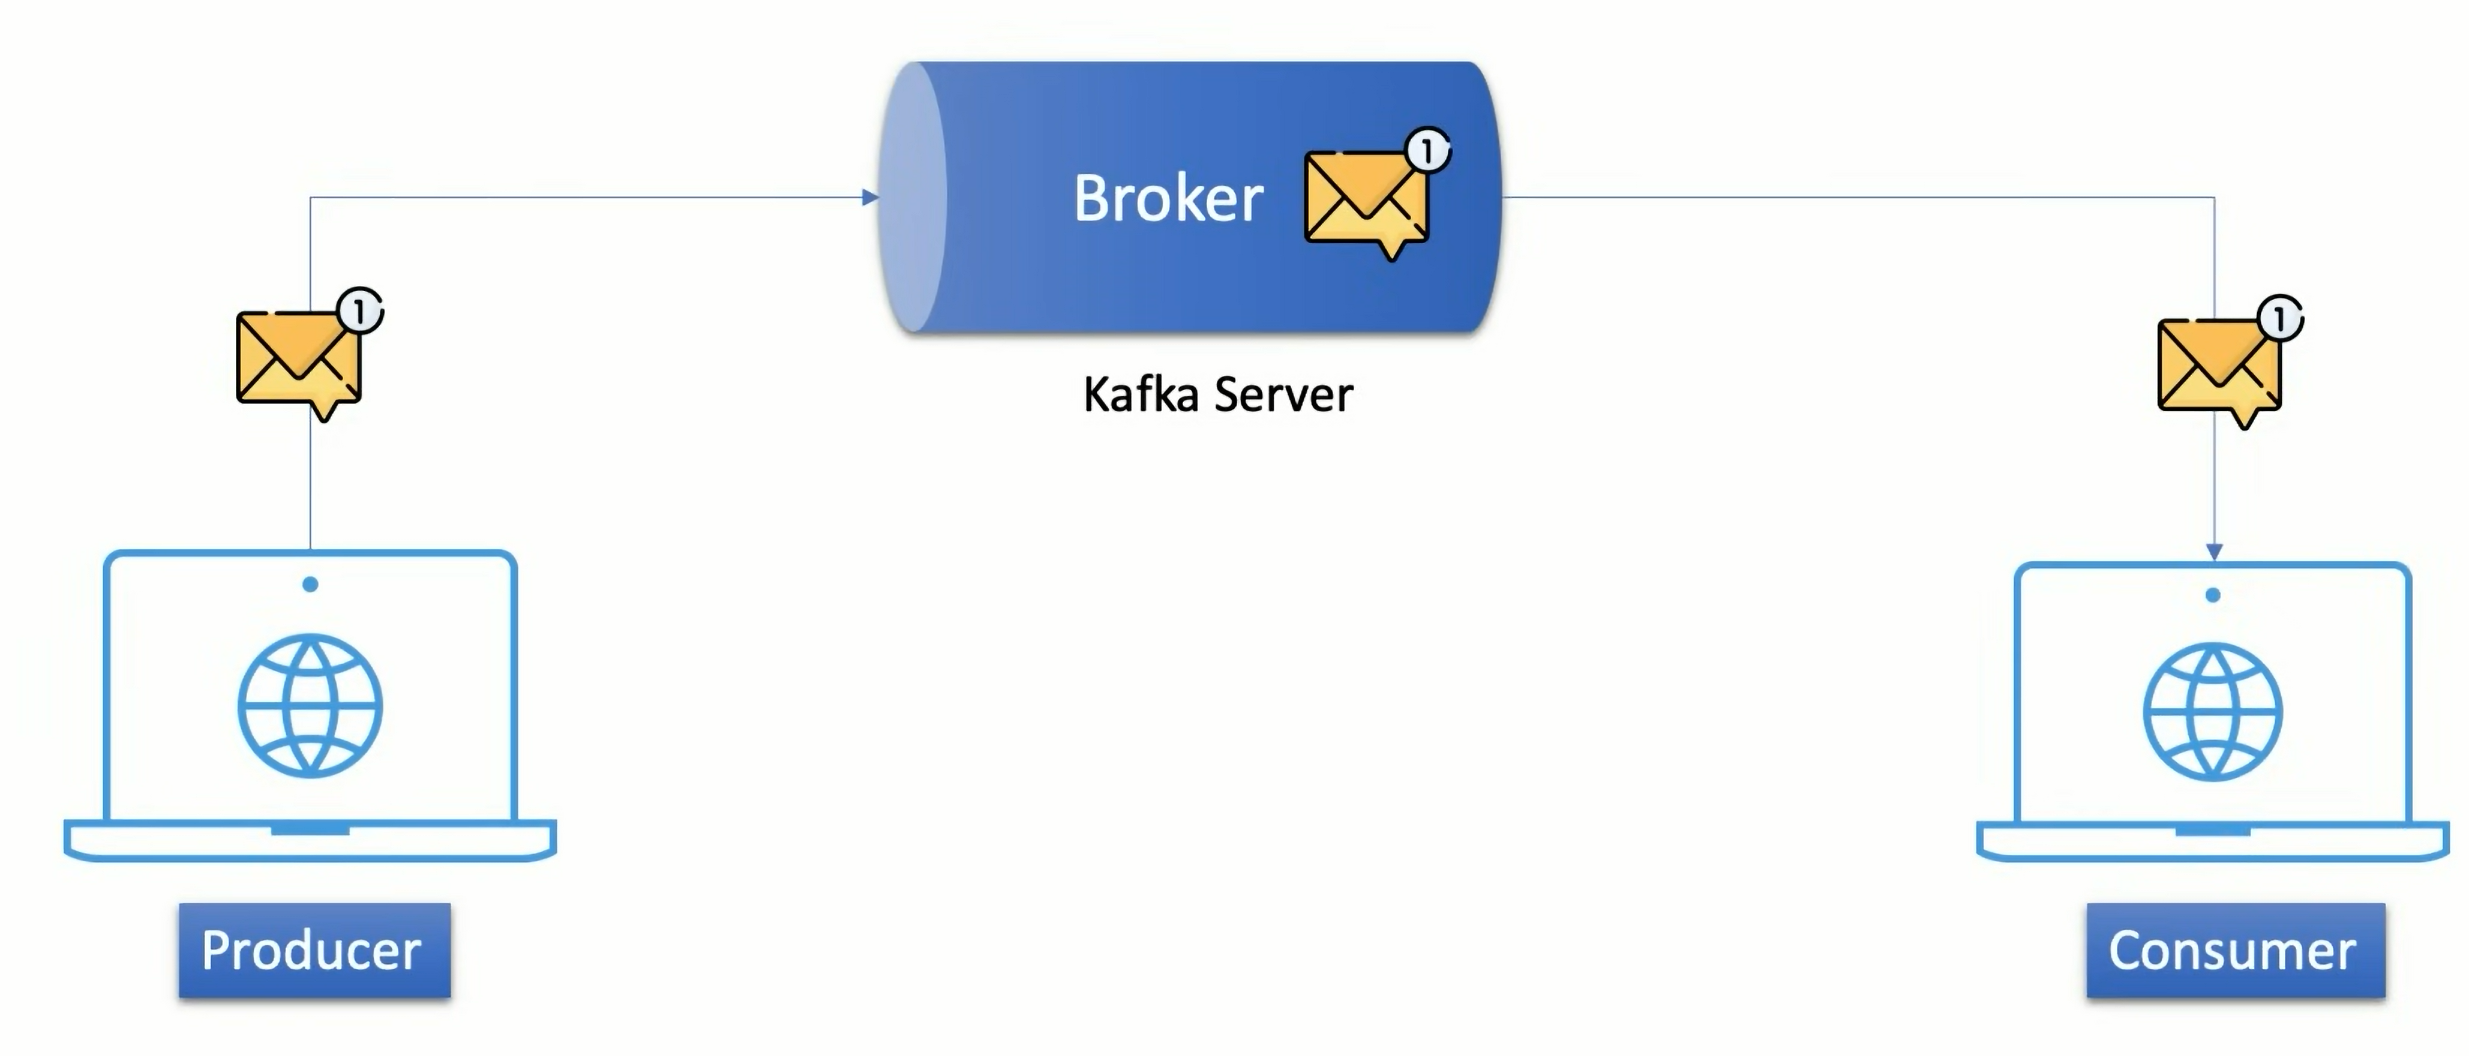
\includegraphics[scale=0.15]{fig/broker.png}
\end{frame}

\begin{frame}{Kafka Components}
  \begin{itemize}
    \item Producer
    \item Consumer
    \item Broker
    \item \hl{Cluster}
    \item Topic
    \item Partitions
    \item Offset
    \item Consumer Groups
    \item Zookeeper
  \end{itemize}
  \begin{tikzpicture}[remember picture, overlay]
    \node[left=3em] at (current page.east)
    {
      
\includegraphics[width=0.35\textwidth]{fig/kafka_logo.png}
    };
  \end{tikzpicture}
\end{frame}

\begin{frame}{Kafka Components}{Cluster}
  \begin{itemize}
    \item There can be one or more brokers in the Kafka cluster.
    \item Its distributed architecture is one of the reasons that made Kafka so popular.
    \item The Brokers is what makes it so resilient, reliable, scalable, and fault-tolerant.
  \end{itemize}
  \vspace*{1em}
  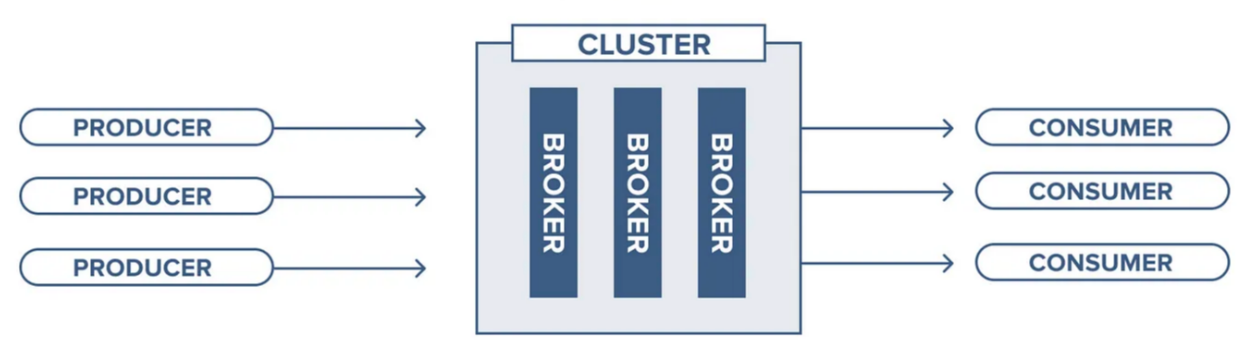
\includegraphics[width=1\textwidth]{fig/cluster.png}
\end{frame}

\begin{frame}{Kafka Components}
  \begin{itemize}
    \item Producer
    \item Consumer
    \item Broker
    \item Cluster
    \item \hl{Topic}
    \item Partitions
    \item Offset
    \item Consumer Groups
    \item Zookeeper
  \end{itemize}
  \begin{tikzpicture}[remember picture, overlay]
    \node[left=3em] at (current page.east)
    {
      
\includegraphics[width=0.35\textwidth]{fig/kafka_logo.png}
    };
  \end{tikzpicture}
\end{frame}

\begin{frame}{Kafka Components}{Topic}
  \begin{itemize}
    \item Specifies the category of the message or the classification of the message.
    \item Consumers can then just respond to the messages that belong to the topics they are listening on.
  \end{itemize}
  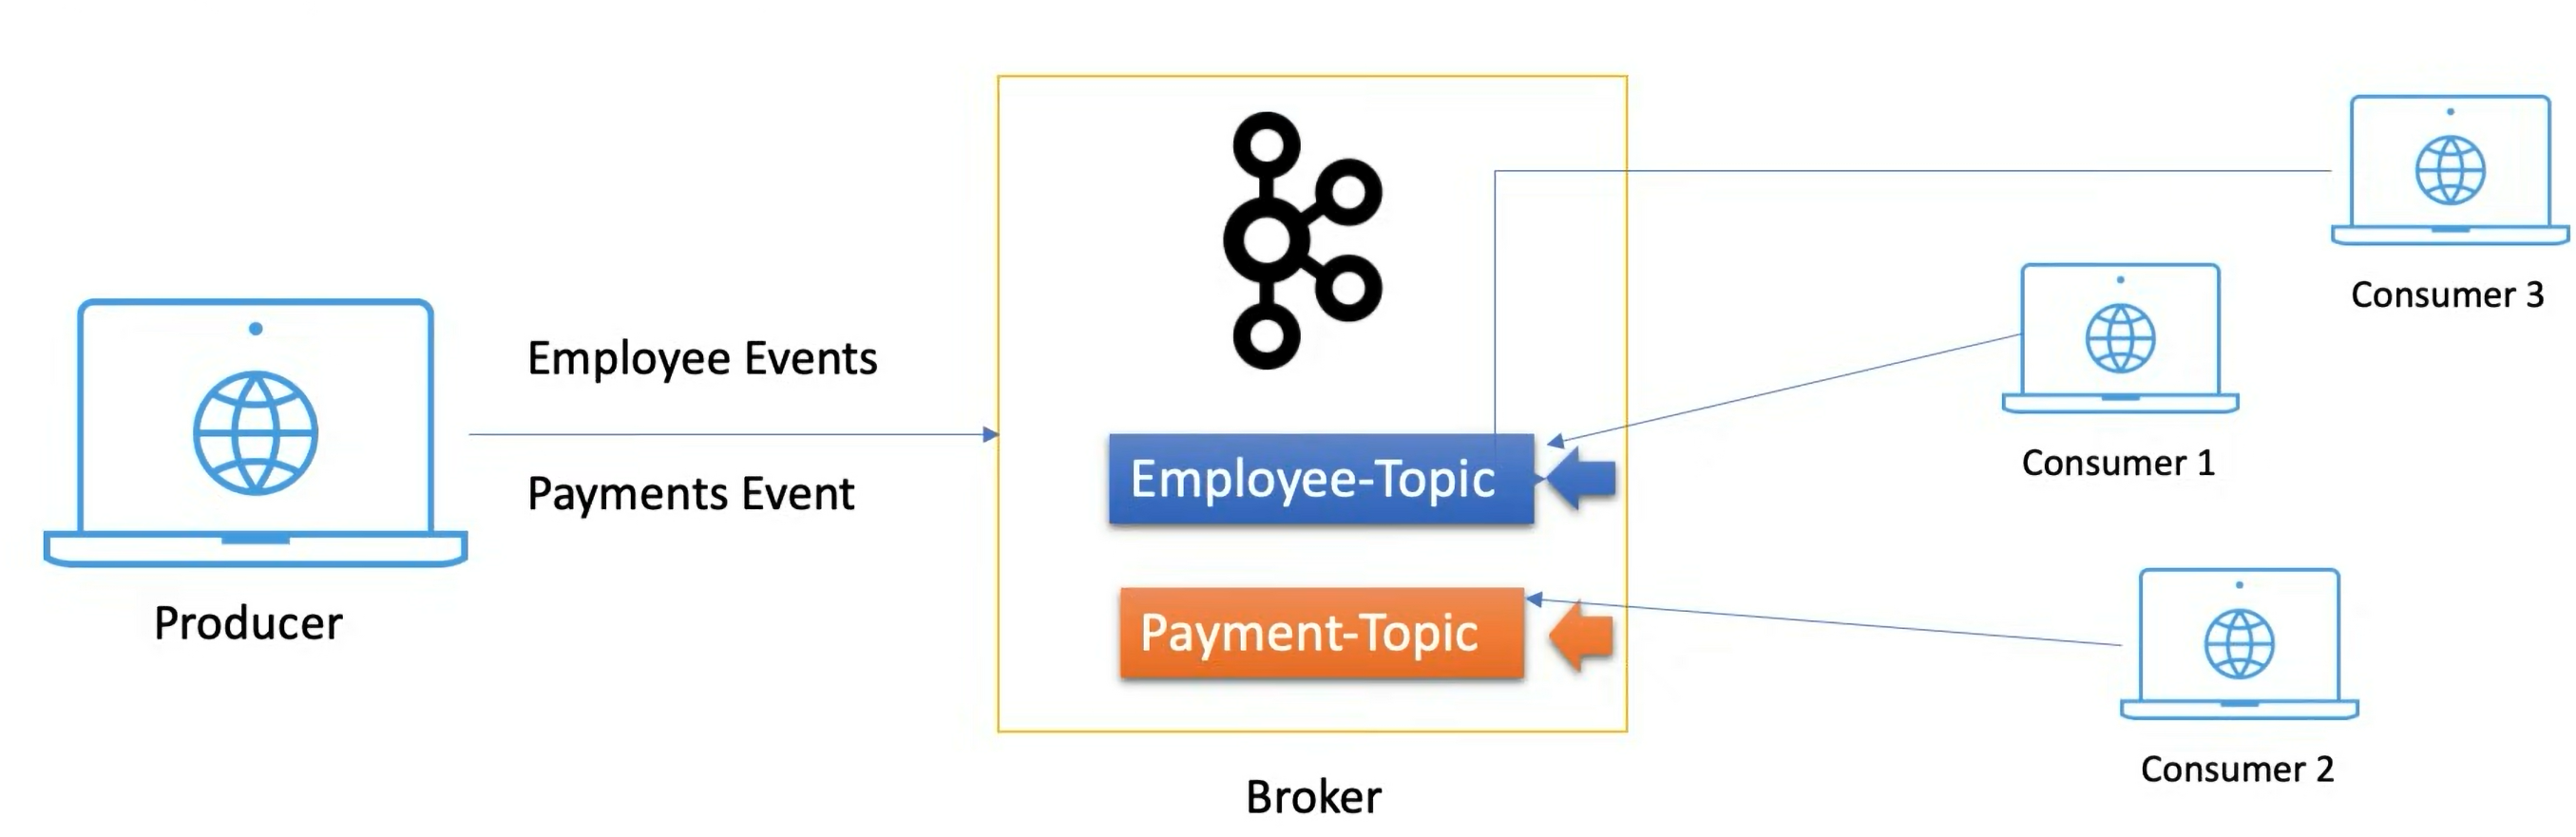
\includegraphics[width=0.98\textwidth]{fig/topic.png}
\end{frame}

\begin{frame}{Kafka Components}
  \begin{itemize}
    \item Producer
    \item Consumer
    \item Broker
    \item Cluster
    \item Topic
    \item \hl{Partitions}
    \item Offset
    \item Consumer Groups
    \item Zookeeper
  \end{itemize}
  \begin{tikzpicture}[remember picture, overlay]
    \node[left=3em] at (current page.east)
    {
      
\includegraphics[width=0.35\textwidth]{fig/kafka_logo.png}
    };
  \end{tikzpicture}
\end{frame}

\begin{frame}{Kafka Components}{Partitions}
  \begin{itemize}
    \item A topic is divided into \textbf{partitions}.
    \item Each topic can have one or more partitions.
    \item We need to specify the number of partitions when creating the topic.
  \end{itemize}
  \hspace*{5em}
  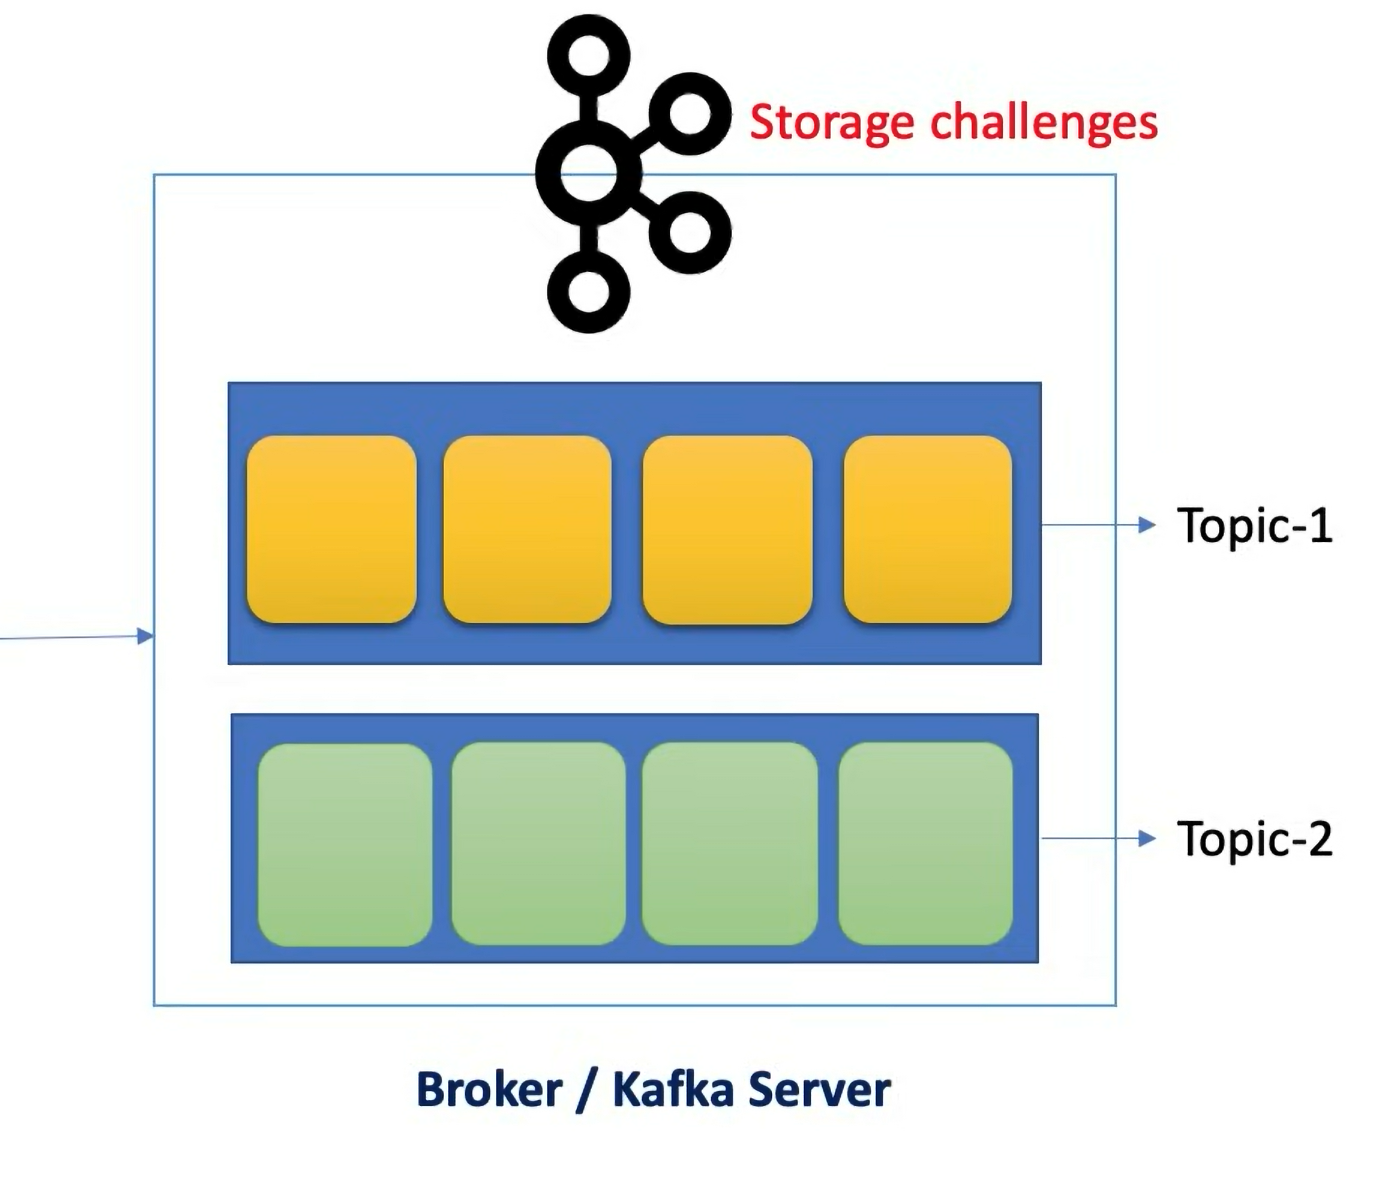
\includegraphics[width=0.57\textwidth]{fig/partitions.png}
\end{frame}
% If we don’t give any key to a message when we’re producing it, by default, 
% the producers will send the message in a round-robin way, each partition will 
% receive a message (even if they are sent by the same producer). Because of that, 
% we aren’t able to guarantee the delivery order at the partition level, if we 
% want to send a message always to the same partition, we need to 
% give a key to our messages. This will ensure that the message will always 
% be sent to the same partition;

\begin{frame}{Kafka Components}
  \begin{itemize}
    \item Producer
    \item Consumer
    \item Broker
    \item Cluster
    \item Topic
    \item Partitions
    \item \hl{Offset}
    \item Consumer Groups
    \item Zookeeper
  \end{itemize}
  \begin{tikzpicture}[remember picture, overlay]
    \node[left=3em] at (current page.east)
    {
      
\includegraphics[width=0.35\textwidth]{fig/kafka_logo.png}
    };
  \end{tikzpicture}
\end{frame}

\begin{frame}{Kafka Components}{Offset}
  \begin{itemize}
    \item Each message will be stored in the broker disk and will receive an \textbf{offset}.
    \item Each partition has its own offsets.
    \item Kafka stores the messages on the disk (like a database).
  \end{itemize}
  \hspace*{1em}
  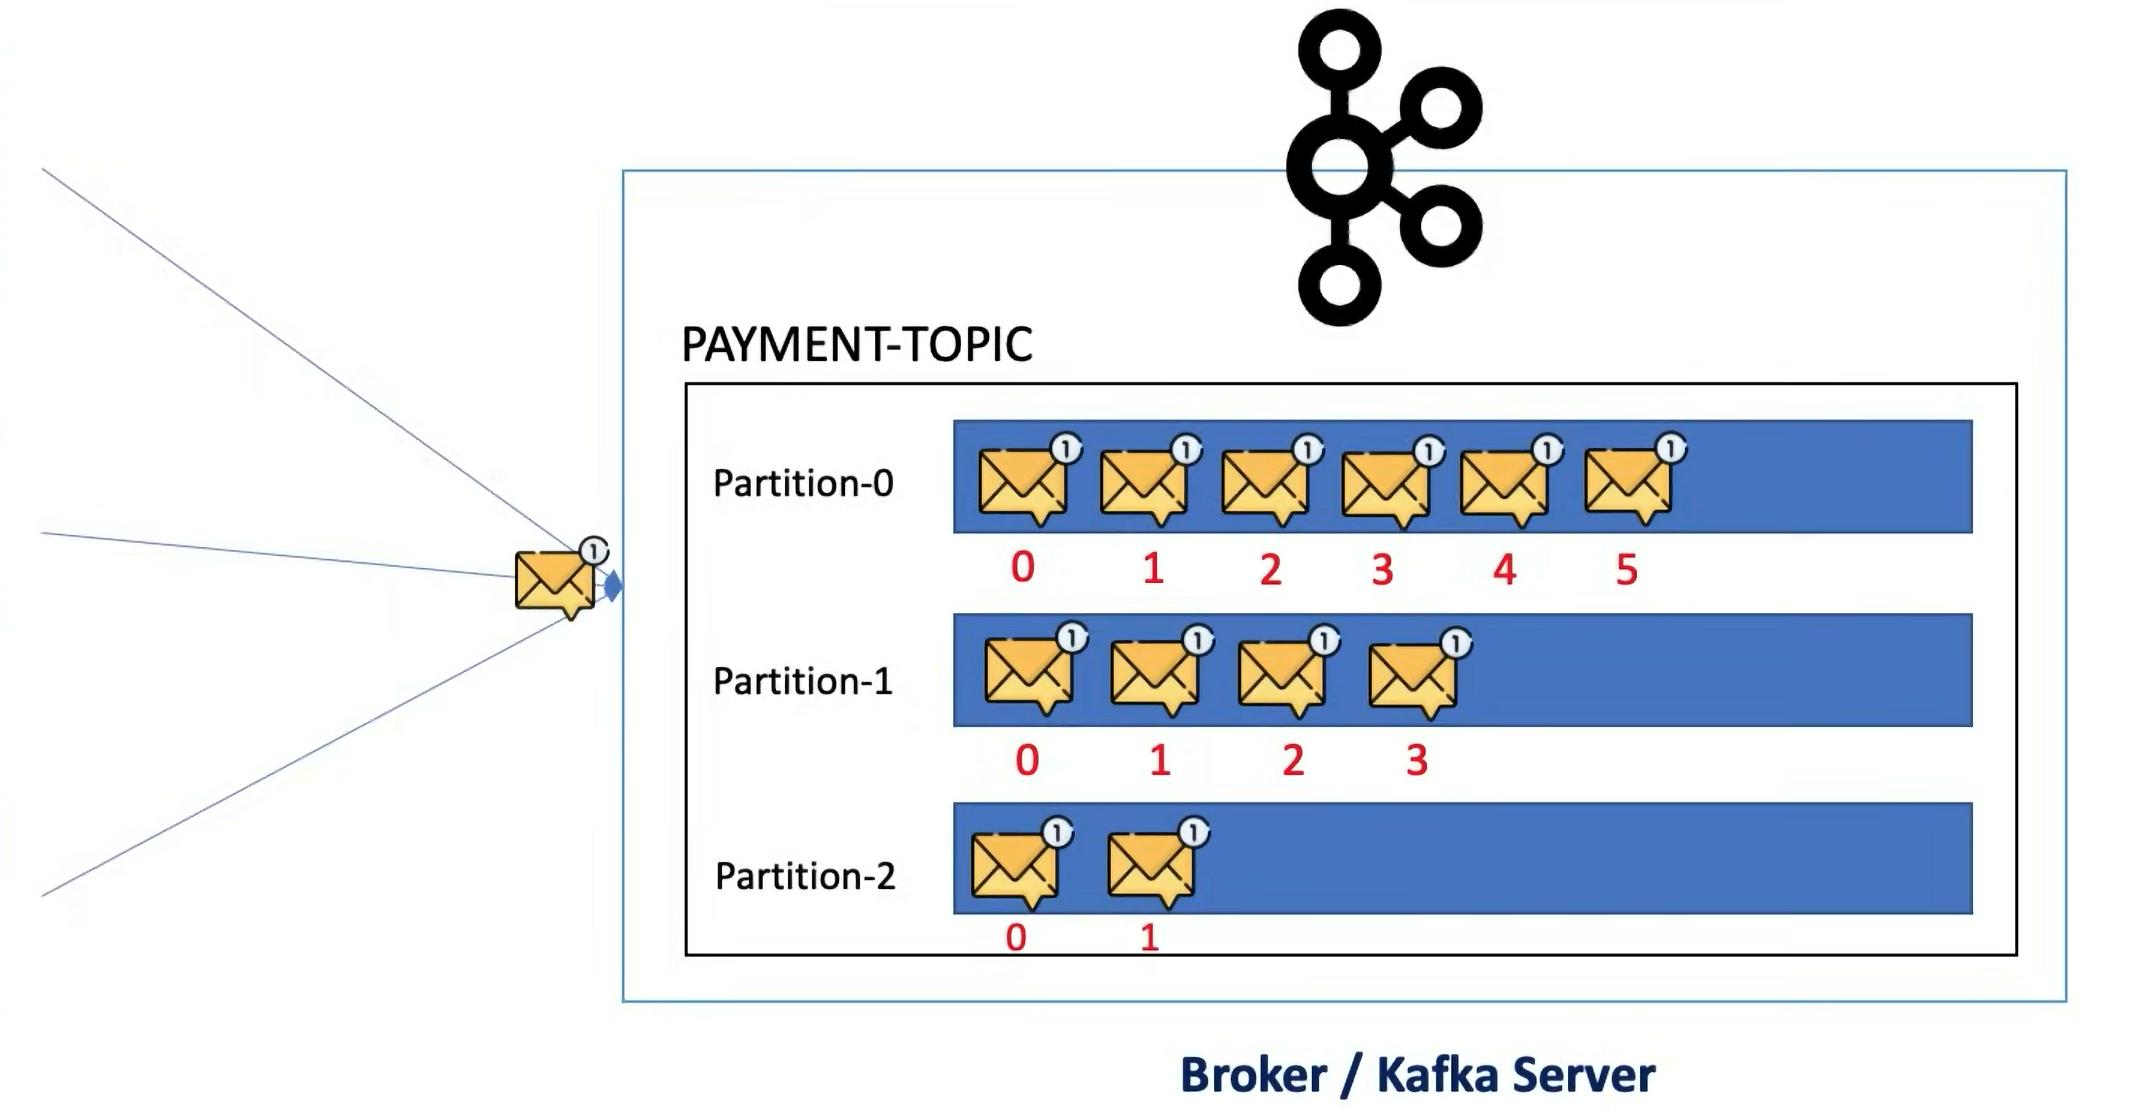
\includegraphics[width=0.85\textwidth]{fig/offset.png}
\end{frame}
% Primarily he consumer keeps the offset value.

\begin{frame}{Kafka Components}
  \begin{itemize}
    \item Producer
    \item Consumer
    \item Broker
    \item Cluster
    \item Topic
    \item Partitions
    \item Offset
    \item \hl{Consumer Groups}
    \item Zookeeper
  \end{itemize}
  \begin{tikzpicture}[remember picture, overlay]
    \node[left=3em] at (current page.east)
    {
      
\includegraphics[width=0.35\textwidth]{fig/kafka_logo.png}
    };
  \end{tikzpicture}
\end{frame}

\begin{frame}{Kafka Components}{Consumer Groups}
  \begin{itemize}
    \item It becomes very costly when a single consumer needs to read from many partitions.
    \item We need some sort of load-balancing, this is where \textbf{consumer groups} enter.
    \item The ideal is to have the same number of consumers in a group that we have as partitions in a topic, in this way, every consumer read from only one.
  \end{itemize}
  \hspace*{4.5em}
  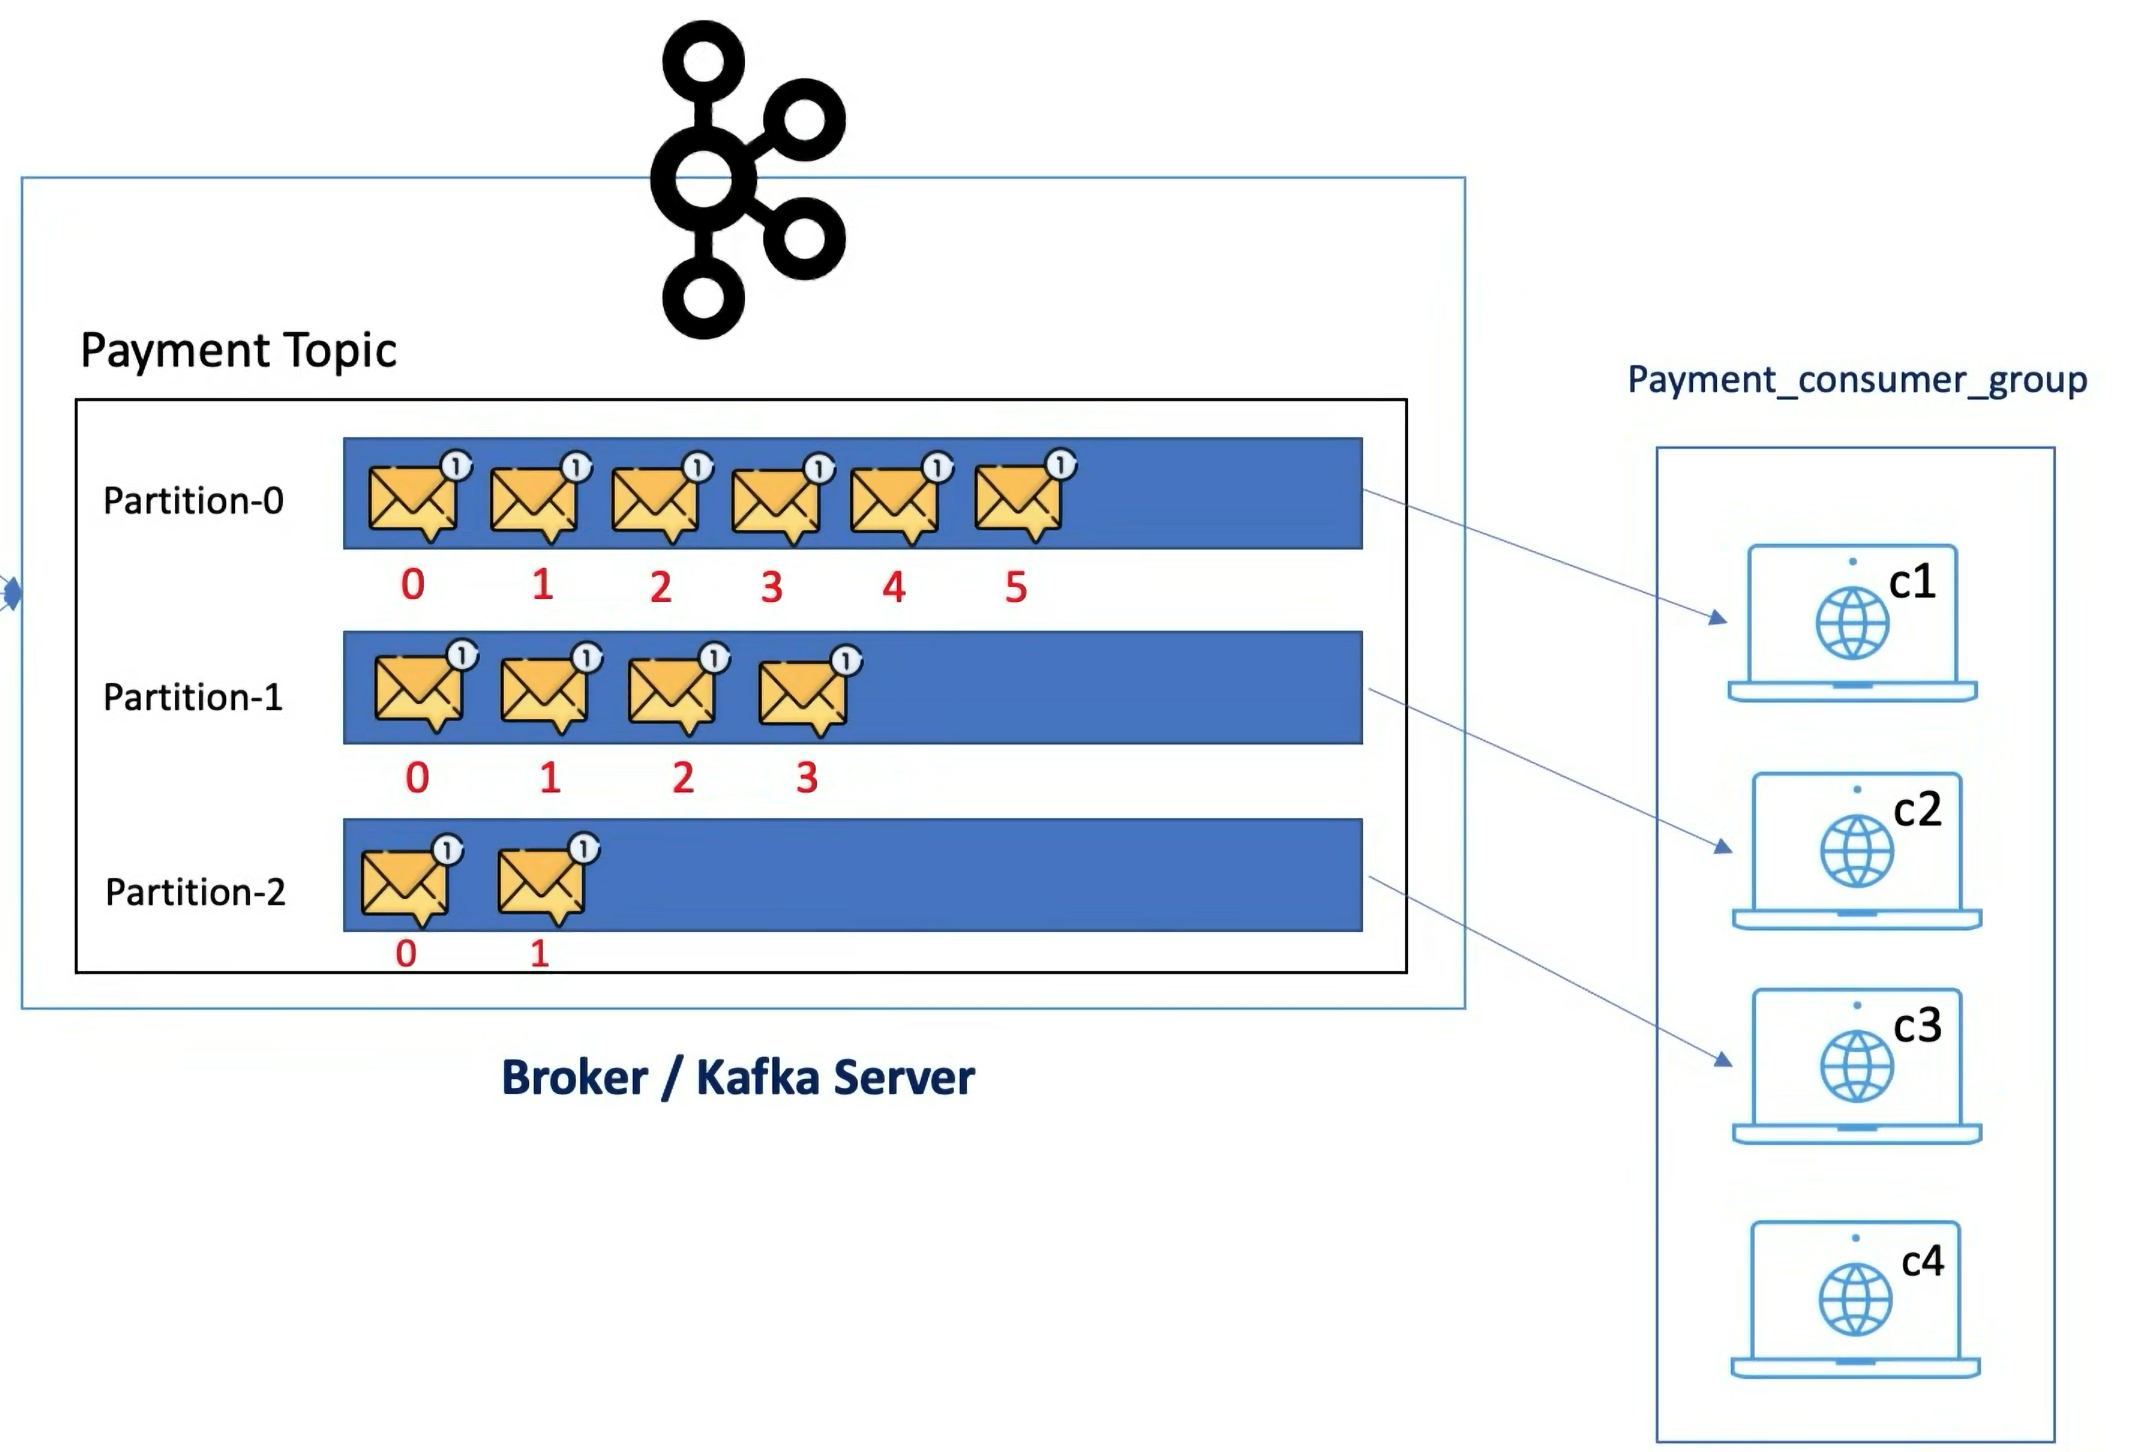
\includegraphics[width=0.65\textwidth]{fig/consumer_group.png}
\end{frame}
% When adding consumers to a group, you need to be careful, if the number of 
% consumers is greater than the number of partitions, some consumers
% will not read from any topic and will stay idle.

\begin{frame}{Kafka Components}
  \begin{itemize}
    \item Producer
    \item Consumer
    \item Broker
    \item Cluster
    \item Topic
    \item Partitions
    \item Offset
    \item Consumer Groups
    \item \hl{Zookeeper}
  \end{itemize}
  \begin{tikzpicture}[remember picture, overlay]
    \node[left=3em] at (current page.east)
    {
      
\includegraphics[width=0.35\textwidth]{fig/kafka_logo.png}
    };
  \end{tikzpicture}
\end{frame}

\begin{frame}{Kafka Components}{Zookeeper}
  \begin{itemize}
    \item \textbf{Zookeeper} is a prerequisite for Kafka.
    \item Kafka is a distributed system, and it uses \textbf{Zookeeper} for coordination and to track the status of Kafka cluster nodes.
    \item \textbf{Zookeeper} also keeps track of Kafka topics, partition, offsets.
          % \item Basically it acts as a manager for the Kafka Cluster.
  \end{itemize}
  \hspace*{2.6em}
  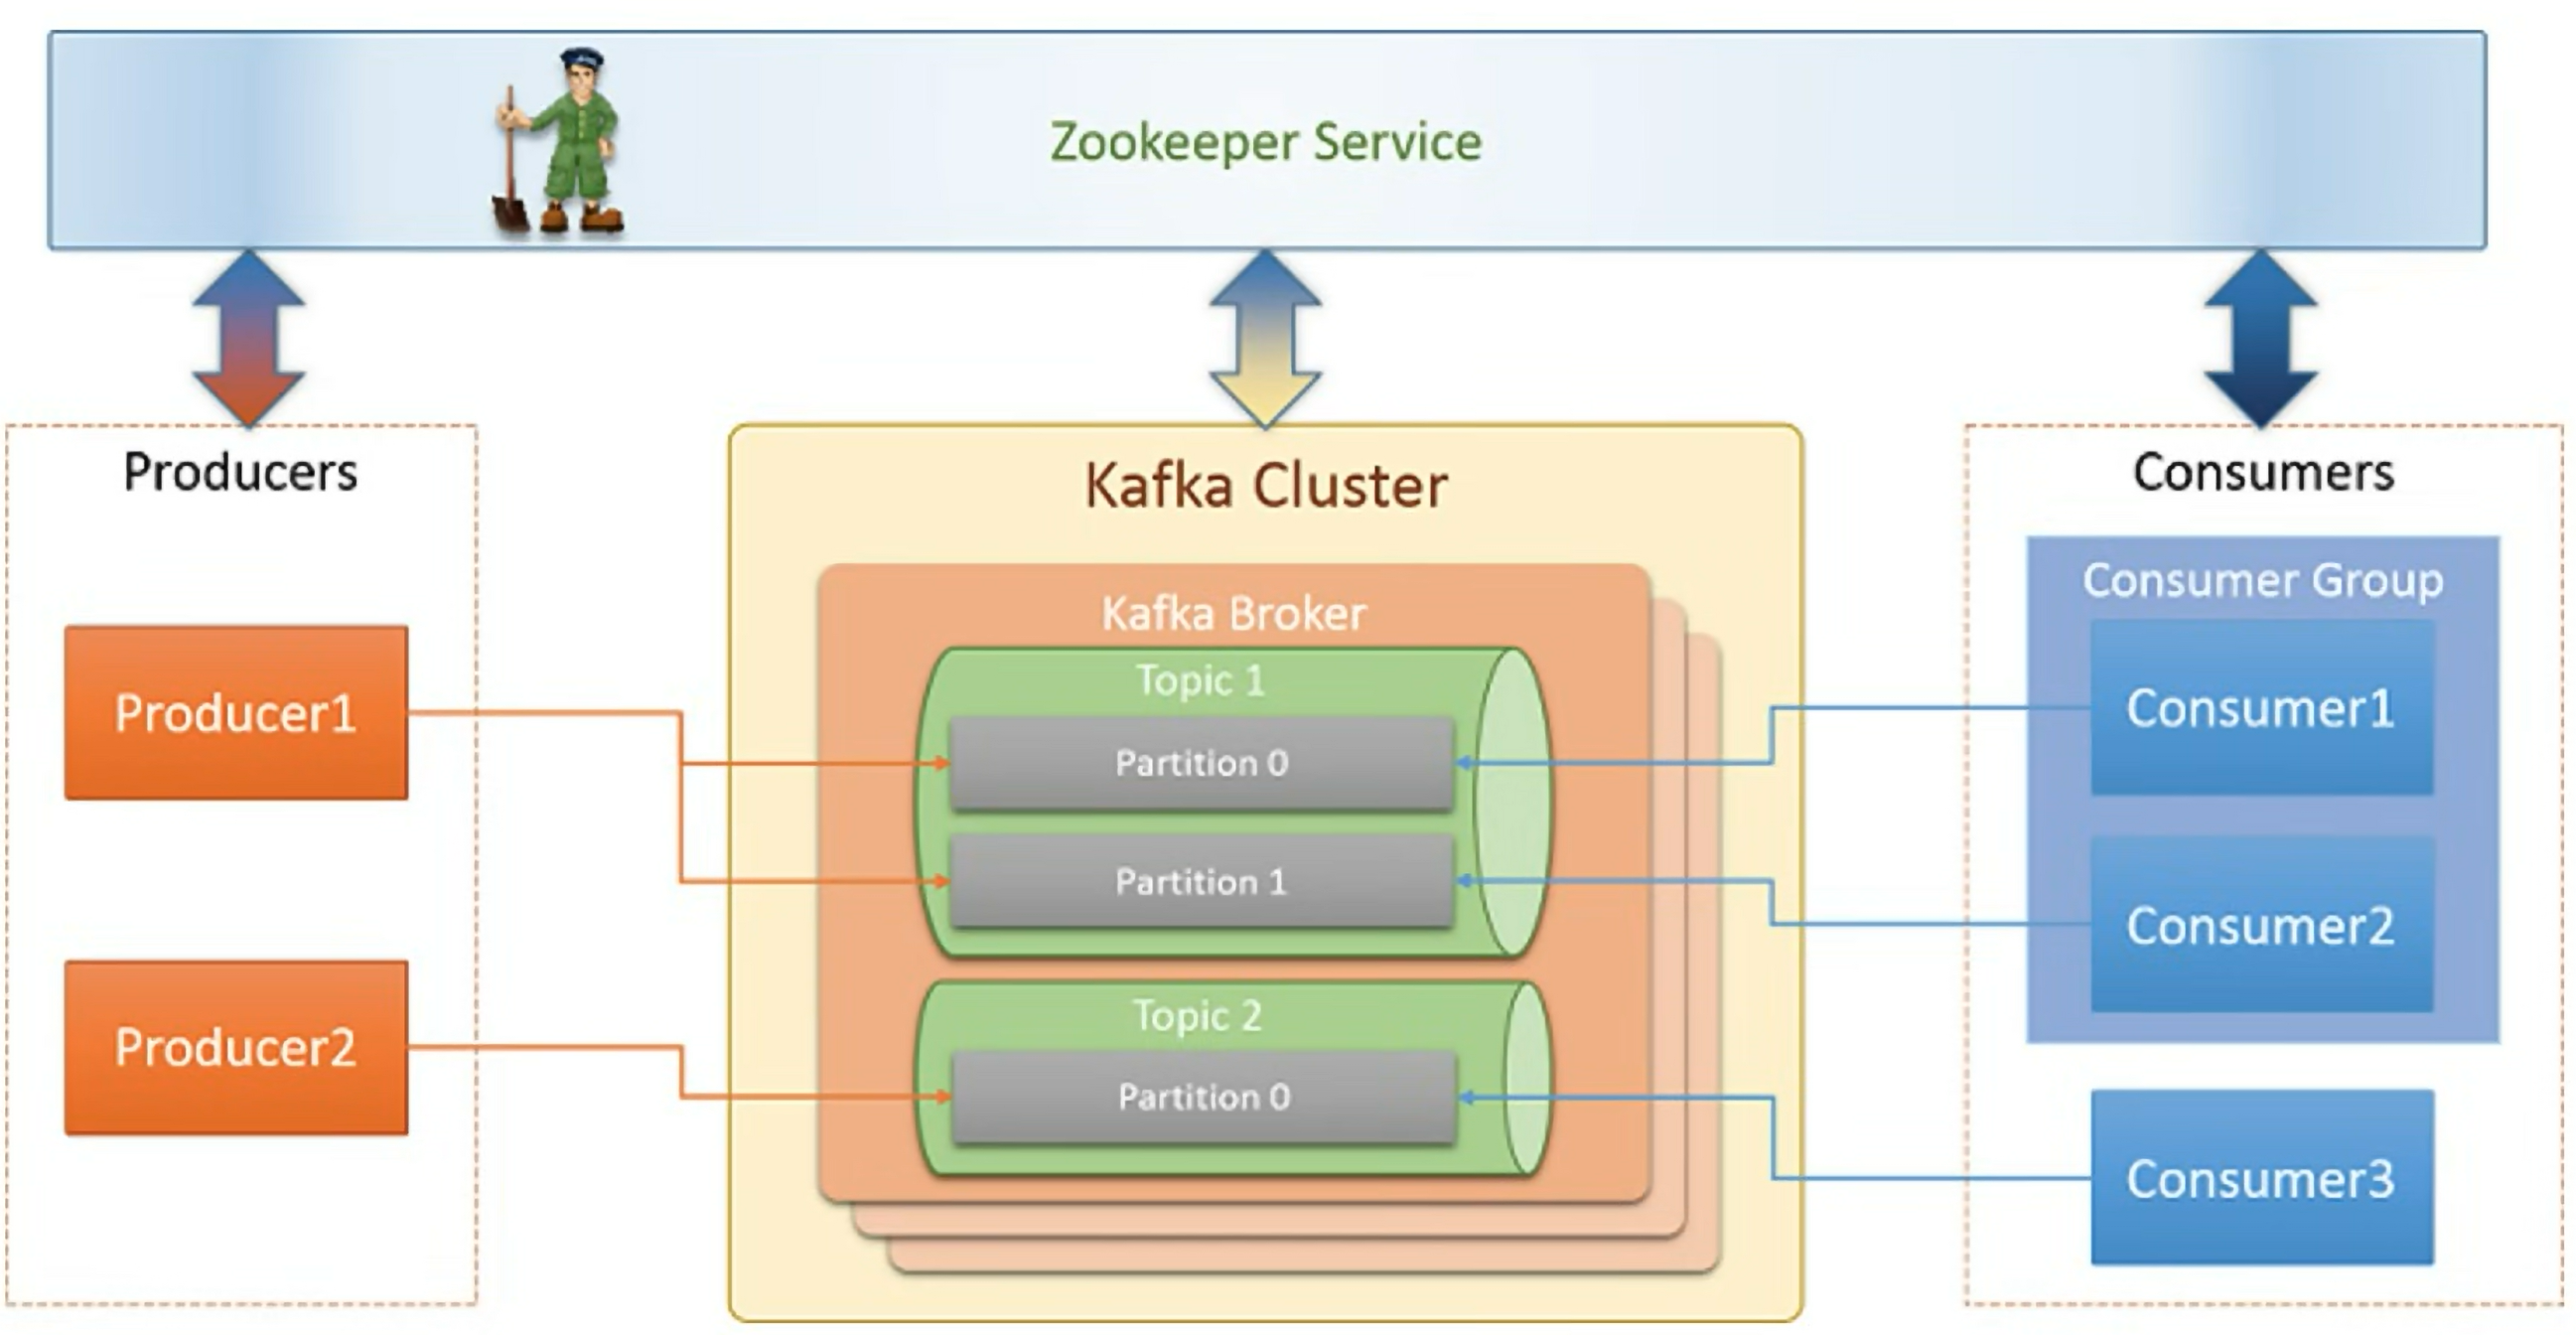
\includegraphics[width=0.84\textwidth]{fig/zookeeper.png}
\end{frame}

\begin{frame}{Internal Architecture}{Partition Leader}
  \begin{itemize}
    \item To ensure the reliability of the cluster, Kafka enters with the concept of the \textbf{Partition Leader}.
    \item Only one leader can exist per partition in all brokers.
    \item The leader is the only one that receives the messages, their replicas will just sync the data.
    \item When a leader goes down, a replica will be automatically elected as a new leader by \textbf{Zookeeper}.
  \end{itemize}
\end{frame}

\begin{frame}{Internal Architecture}{Acknowledgment}
  \begin{itemize}
    \item The \textbf{Acknowledgment (ack)} is a confirmation that the message was delivered.
    \item In Kafka we can configure this ack in three different levels:
          \vspace*{1.2em}
    \item \textbf{ack = 0}: We dont want to receive ack from Kafka.
    \item \textbf{ack = 1}: Default configuration, we want to receive an ack from the partition leader.
    \item \textbf{ack = all}: We want to receive confirmation from partition leader and their replicas as well.
  \end{itemize}
\end{frame}


\section[Kafka vs RabbitMQ]{Kafka vs RabbitMQ}

\begin{frame}{Kafka vs RabbitMQ}{part 1}
  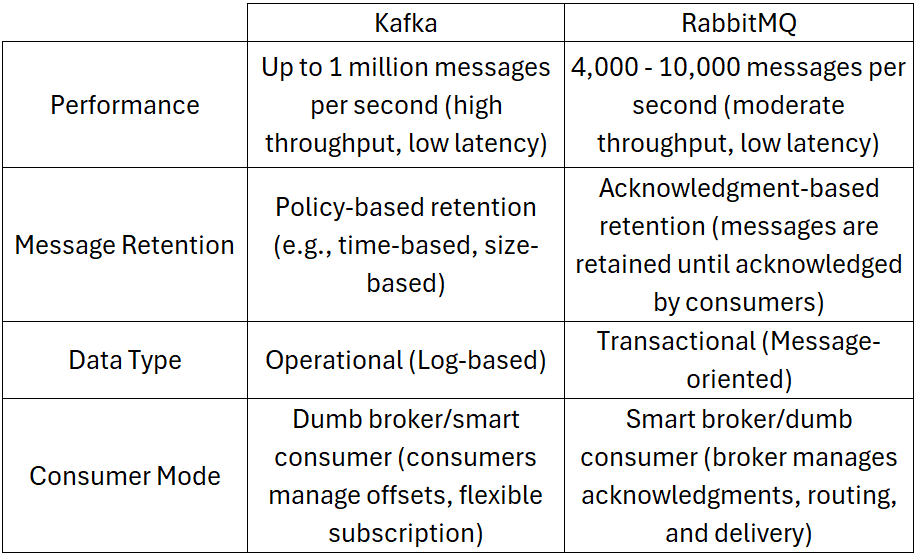
\includegraphics[width=1.02\textwidth]{fig/vs1.png}
\end{frame}

\begin{frame}{Kafka vs RabbitMQ}{part 2}
  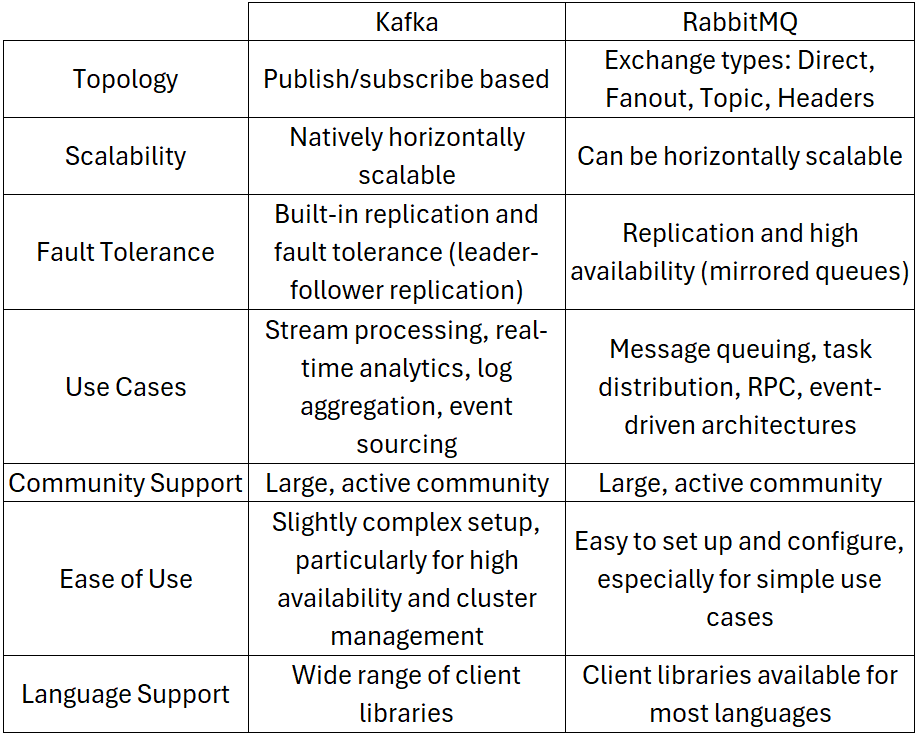
\includegraphics[width=0.99\textwidth]{fig/vs2.png}
\end{frame}


\section[Hotel Reservations example]{Hotel Reservations example}

% \begin{frame}{Hotel Reservations}
%   \begin{itemize}
%     \item Demo:
%   \end{itemize}
% \end{frame}

\begin{frame}{Demo: Hotel Reservations}{System Architecture}
  \begin{tikzpicture}[remember picture, overlay]
    \node[right=4.02em] at (current page.185)
    {
      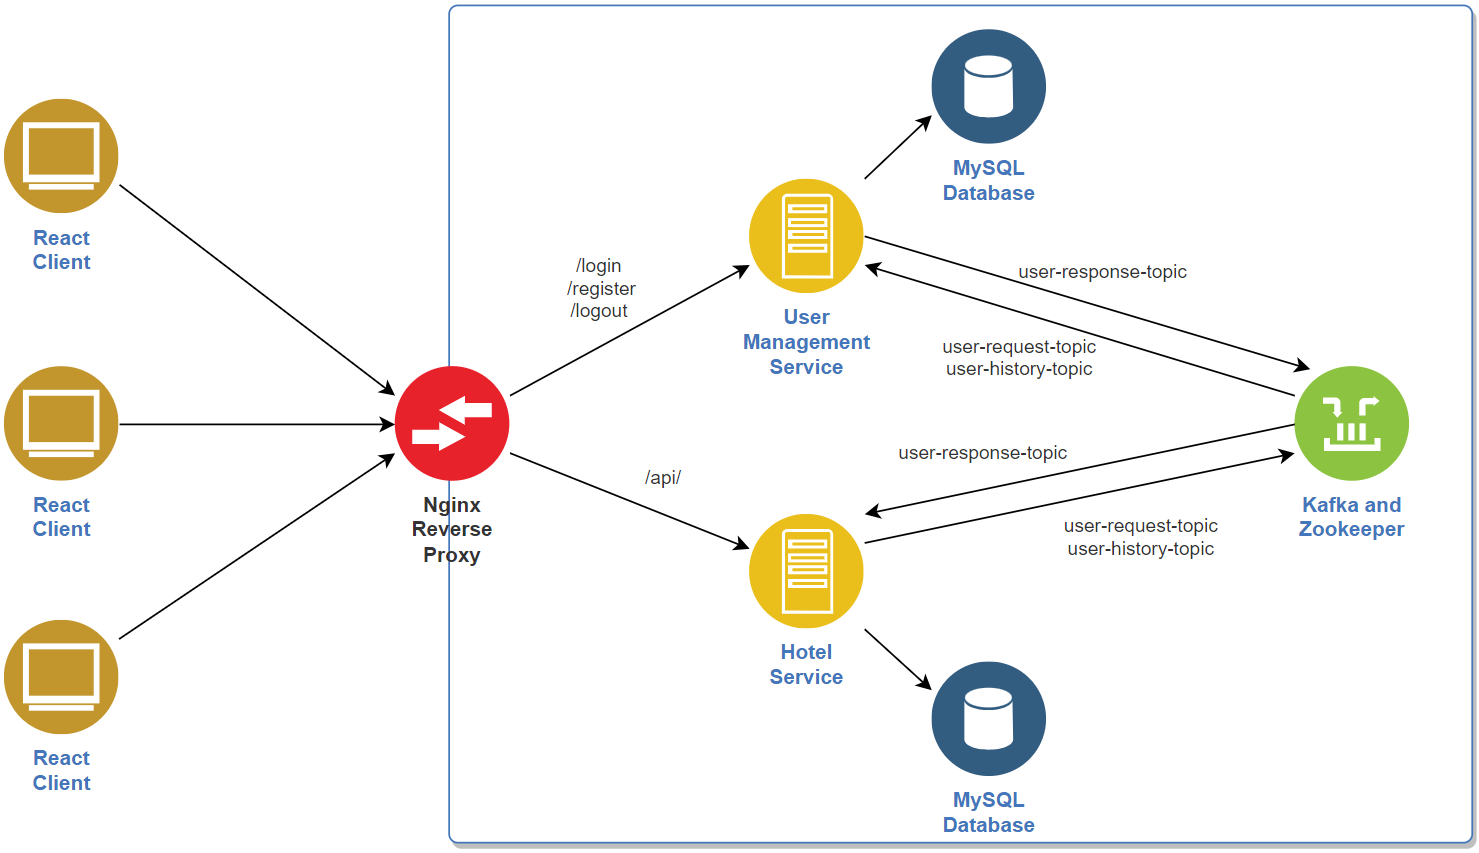
\includegraphics[width=1.09\textwidth]{fig/image.png}
    };
  \end{tikzpicture}
\end{frame}


\section[References]{References}

\begin{frame}{References}
  \begin{itemize}
    % \item \href{https://kafka.apache.org/intro}{kafka.apache.org/intro}
    \item \url{https://kafka.apache.org/intro}
    \item \url{https://www.cloudkarafka.com/blog/2016-11-30-part1-kafka-for-beginners-what-is-apache-kafka.html}
    \item \url{https://fullcycle.com.br/apache-kafka-trabalhando-com-mensageria-e-real-time/}
    \item \url{https://www.educba.com/kafka-replication/}
    \item \url{https://www.javatpoint.com/apache-kafka-producer}
    \item \url{https://docs.cloudera.com/cdp-private-cloud-base/latest/kafka-developing-applications/topics/kafka-develop-groups-fetching.html}
  \end{itemize}
\end{frame}

\end{document}
